\section{形变捕捉技术}
随着深度相机,如Kinect\cite{microsoft_kinect}的普及,产生了很多的静态三维重建的相关工作,
如KinectFusion\cite{newcombe2011kinectfusion}。
在这些研究的基础上,很多研究者希望更进一步,利用深度相机实现动态场景的捕捉。
很多动态场景捕捉的相关工作都关注在人体特定部分的形变捕捉。
这些人体的部位往往具有特殊的形状和既定的运动模式,
这些运动模式可以是通过观察总结的也可以是认为规定的。
有很多高精度高效率的的工作聚焦于人脸\cite{cao20133d}\cite{li2013realtime}、
手\cite{oikonomidis2011efficient}\cite{qian2014realtime}、
身体\cite{taylor2012vitruvian}或铰接件\cite{schmidt2014dart}\cite{ye2014real}的形变。
% \begin{figure}[h]
%     \centering
%     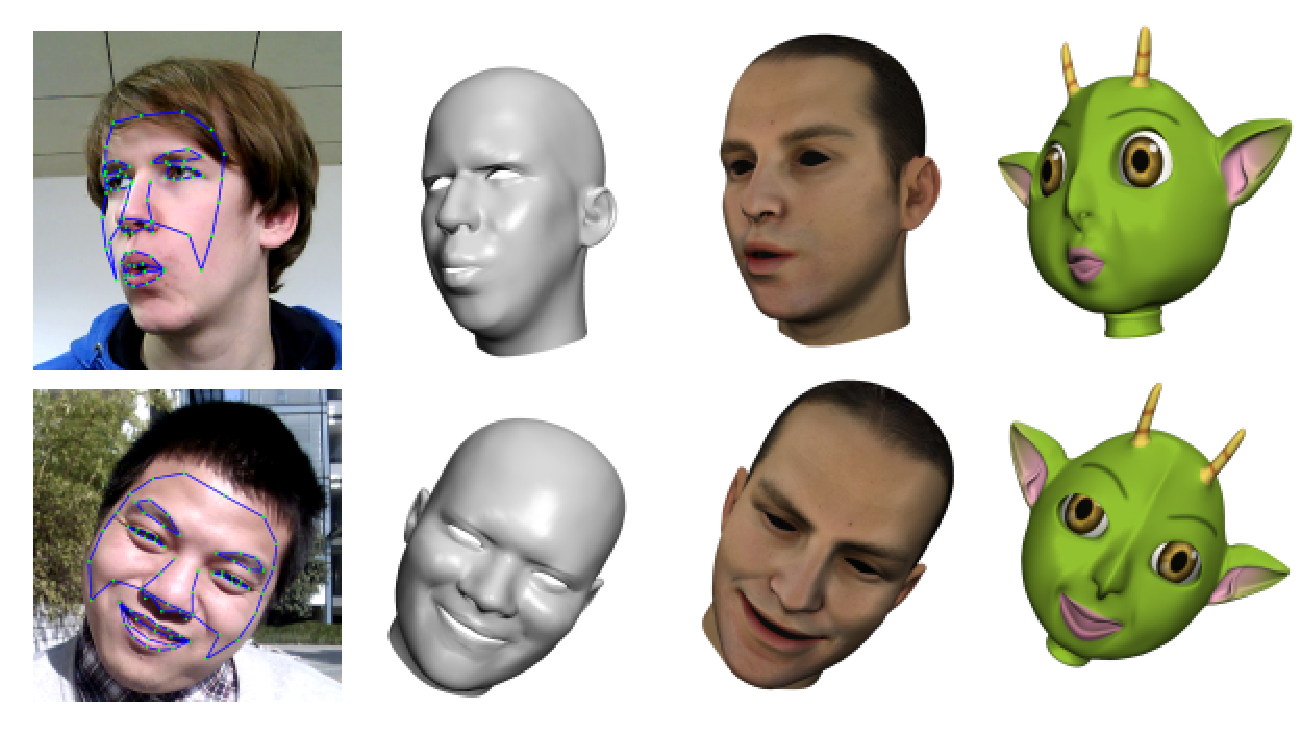
\includegraphics[width = 0.7\textwidth]{./Pictures/facial_animation.eps}
%     \caption{Cao的实时人脸动画捕捉系统}
%     \label{facial_animation}
% \end{figure}
\begin{figure}[h]
    \centering
    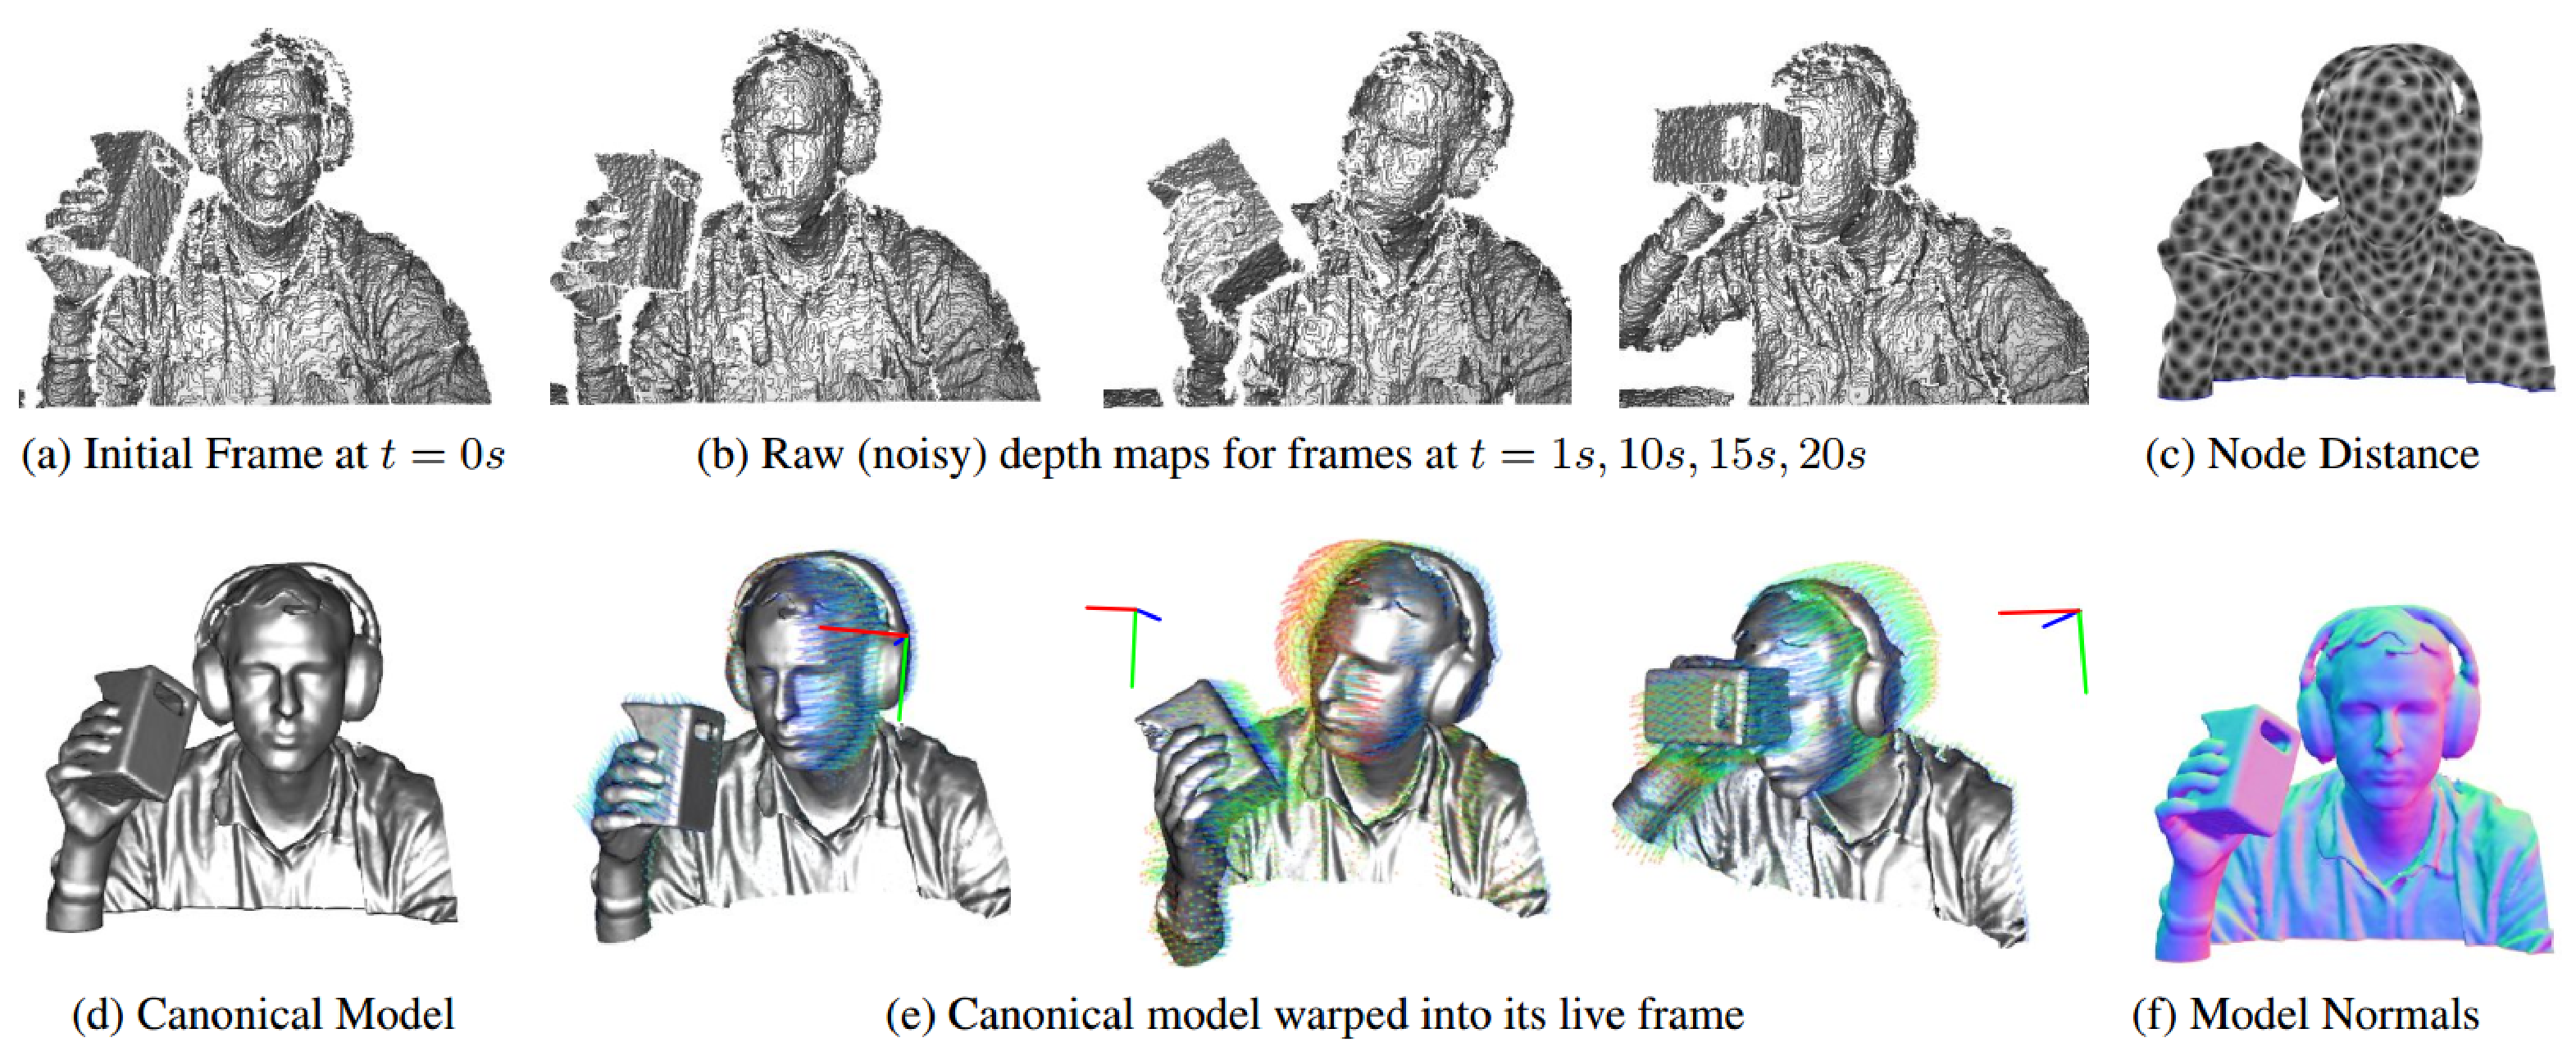
\includegraphics[width = \textwidth]{./Pictures/dynamic_fusion.eps}
    \caption{DynamicFusion——一个实时非刚体SLAM系统}
    \label{dynamic_fusion}
\end{figure}

此外,也有很多研究工作直接捕捉更为通用的网格模型的形变。
Li的工作\cite{li2009robust}通过扫描获取物体模型,
并用一个低分辨率的模型作为先验的形变模板来追踪物体大致的形变,
并通过非刚体重建获得高频的几何细节。
后来,Zollh{\"o}fer\cite{zollhofer2014real}的工作使用了类似的技术,借助GPU加速,
给出了一个高效的实时形变捕捉系统。
在这个系统实时的维护了一个高分辨率的刚体模型,作为非刚体捕捉的先验,以提高形变捕捉的效率。
受到了这些工作的启发,
DynamicFusion\cite{newcombe2015dynamicfusion}给出了一个能够捕捉形变并重建非刚体场景的SLAM系统。
与章节\ref{reconstruction}中所描述的三维重建系统类似,
DynamicFusion维护着一个基于TSDF的静态模型(Canonical Model)。
此外,该工作还维护了一个描述模型形变的非刚体形变场(Non-rigid Warp Field),
用以描述了模型的形变,如图\ref{dynamic_fusion}。
本文的形变捕捉系统主要参考的就是该工作的形变捕捉框架。
